% Cart-pole schematic for the Back2Basics notes.
% Build:  scripts/build-figures.sh   (pdflatex -> dvisvgm -> themed SVG)
%
% Convention drawn here (matches the hand-derived notes):
%   - point mass m suspended a distance l below the cart's centre
%   - theta measured from the DOWNWARD vertical, positive toward +x
%   - x measured along the rail from the origin to the cart's centre
%   - F applied horizontally to the cart, positive toward +x
\documentclass[tikz,border=6pt]{standalone}
\usepackage{amsmath}
\usetikzlibrary{arrows.meta,calc,positioning}

\begin{document}
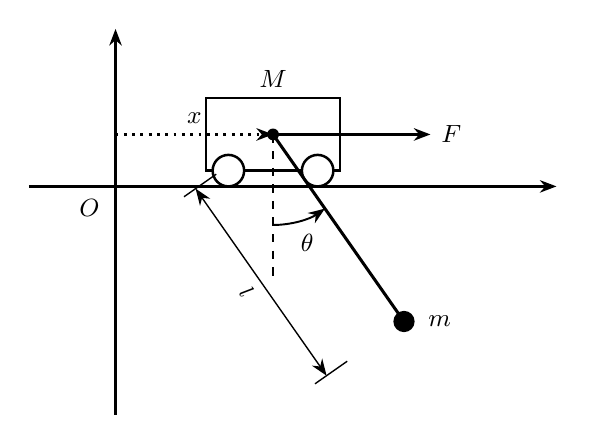
\begin{tikzpicture}[
    >={Stealth[length=6pt]},
    line width=0.9pt,
    every node/.style={font=\small},
    dim/.style={line width=0.5pt},
  ]

  % ---- geometry ------------------------------------------------------
  \def\polang{35}      % angle from the downward vertical, positive toward +x
  \def\lpole{2.9}      % pivot to point mass
  \def\cartx{2.0}      % cart position along the rail
  \def\cartw{1.7}
  \def\carth{0.92}
  \def\wrad{0.20}

  \pgfmathsetmacro{\ypiv}{\wrad+\carth/2}
  \pgfmathsetmacro{\poldir}{-90+\polang}    % pole direction from +x axis

  \coordinate (P) at (\cartx, \ypiv);                  % pivot = cart centre
  \coordinate (T) at ($(P)+(\poldir:\lpole)$);         % point mass

  % ---- axes ----------------------------------------------------------
  \draw[->] (0,-2.9) -- (0,2.0);                       % vertical reference
  \draw[->] (-1.1,0) -- (5.6,0) node[below right]{};   % rail
  \node[below left=1pt and 2pt] at (0,0) {$O$};

  % ---- cart ----------------------------------------------------------
  \draw[fill=white] (\cartx-\cartw/2, \wrad)
    rectangle (\cartx+\cartw/2, \wrad+\carth);
  \node[above] at (\cartx, \wrad+\carth) {$M$};
  \draw[fill=white] (\cartx-\cartw/3, \wrad) circle (\wrad);
  \draw[fill=white] (\cartx+\cartw/3, \wrad) circle (\wrad);

  % ---- x to the cart centre, continuing into F -----------------------
  \draw[->,dotted,line width=1.0pt] (0,\ypiv) -- (P) node[midway,above,font=\small]{$x$};
  \draw[->,line width=1.2pt] (P) -- ++(2.0,0) node[right]{$F$};

  % ---- downward vertical reference and theta -------------------------
  \draw[dashed,line width=0.6pt] (P) -- ++(0,-0.62*\lpole);
  \draw[->,line width=0.7pt] ($(P)+(-90:1.15)$) arc (-90:\poldir:1.15);
  \node at ($(P)+(-90+\polang/2:1.45)$) {$\theta$};

  % ---- pole and point mass -------------------------------------------
  \draw[line width=1.1pt] (P) -- (T);
  \fill (P) circle (0.075);
  \fill (T) circle (0.135);
  \node[right=5pt] at (T) {$m$};

  % l, dimensioned along the pole's upper-right side
  \pgfmathsetmacro{\poleperp}{\poldir-90}
  \pgfmathsetmacro{\loff}{1.2}
  \draw[dim] ($(P)+(\poleperp:\loff-0.32)$) -- ($(P)+(\poleperp:\loff+0.18)$);
  \draw[dim] ($(T)+(\poleperp:\loff-0.32)$) -- ($(T)+(\poleperp:\loff+0.18)$);
  \draw[dim,<->] ($(P)+(\poleperp:\loff)$) -- ($(T)+(\poleperp:\loff)$)
    node[midway,sloped,below,font=\footnotesize] {$l$};

\end{tikzpicture}
\end{document}
